\documentclass[12pt]{article}

\usepackage[a4paper,margin=1in]{geometry}
\usepackage{amsmath,amssymb}
\usepackage{newtxtext,newtxmath} % Times-style font
\usepackage{fancyhdr}
\usepackage{listings}
\usepackage{graphicx}
\usepackage{float}
\usepackage{algorithm}
\usepackage{algpseudocode}
\usepackage{xcolor}
\usepackage{booktabs}
\usepackage{array}

\setlength{\textfloatsep}{10pt}
\setlength{\floatsep}{10pt}

\setlength{\parindent}{0pt}
\setlength{\parskip}{5pt}

% Keep entire document at 12 pt
\AtBeginDocument{
    \fontsize{12pt}{14pt}\selectfont
}

\lstdefinestyle{code}{
    language=Python,
    basicstyle=\ttfamily\fontsize{9.5pt}{11.5pt}\selectfont,
    breaklines=true,
    breakatwhitespace=false,
    frame=single,
    numbers=left,
    numberstyle=\tiny\color{gray},
    keywordstyle=\color{blue},
    commentstyle=\color{gray},
    stringstyle=\color{green!50!black},
    columns=fullflexible,
    keepspaces=true,
    showstringspaces=false
}

\lstdefinestyle{output}{
    basicstyle=\ttfamily\fontsize{9.5pt}{11.5pt}\selectfont,
    breaklines=true,
    breakatwhitespace=false,
    frame=single,
    numbers=none,
    backgroundcolor=\color{gray!6},
    columns=fullflexible,
    keepspaces=true,
    showstringspaces=false
}

% ------------------------------------------------
% Header
% ------------------------------------------------

\pagestyle{fancy}
\fancyhf{}

\fancyhead[L]{Name: Kishan Sahu{\hspace{6cm}}}
\fancyhead[R]{Enrollment No.: P26DS017}

\renewcommand{\headrulewidth}{0.4pt}
\setlength{\headheight}{15pt}

\begin{document}

% ------------------------------------------------
% TITLE
% ------------------------------------------------

\begin{center}
\textbf{Computer Science and Engineering Department, SVNIT, Surat}\\
\textbf{M.Tech. I -- Semester I}\\
\textbf{Computer Vision and Image Processing (CSCS111/CSDS119)}\\
\textbf{Lab Assignment 7}\\
\textbf{Radiometry and Image Formation}
\end{center}
\vspace{-4pt}
\hrule
\vspace{6pt}

\section*{Overview}
This laboratory report investigates the fundamental principles of radiometry, surface reflectance mechanisms, optical sensor image formation, and comparative analysis of scenes under direct versus shadowed illumination. All simulations are implemented in Python using standard scientific libraries. In accordance with the assignment instructions, Questions 4 and 5 from Part A are omitted.

% ==============================================================
\section*{Part A: Radiometry and Image Formation}
% ==============================================================

\subsection*{1. Received Illumination vs. Surface Area and Distance}
\textbf{Principle:} For a point radiation source of intensity $I$ (in W/sr), the irradiance $E$ received by a surface normal to the beam at distance $d$ obeys the Inverse Square Law:
\begin{equation}
E = \frac{I}{d^2} \quad [\text{W/m}^2 \text{ or Lux}]
\end{equation}
The total received radiant flux $\Phi$ collected by a receiver of area $A$ is:
\begin{equation}
\Phi = E \cdot A = \frac{I \cdot A}{d^2} \quad [\text{Watts or Lumens}]
\end{equation}

\begin{lstlisting}[style=code]
import numpy as np
import matplotlib.pyplot as plt

I = 100.0  # Source intensity (W/sr)
d = np.linspace(1.0, 10.0, 100)
areas = [0.5, 1.0, 2.0, 4.0]

plt.figure(figsize=(10, 3.8))
plt.subplot(1, 2, 1)
plt.plot(d, I / (d**2), 'b-', lw=2)
plt.title("Irradiance vs. Distance (E = I / d^2)")
plt.xlabel("Distance d (m)"); plt.ylabel("Irradiance E (W/m^2)"); plt.grid(True)

plt.subplot(1, 2, 2)
for A in areas:
    plt.plot(d, (I * A) / (d**2), lw=1.8, label=f"Area = {A} m^2")
plt.title("Received Flux vs. Distance (Phi = I*A / d^2)")
plt.xlabel("Distance d (m)"); plt.ylabel("Total Flux Phi (Watts)"); plt.legend(); plt.grid(True)
plt.tight_layout()
\end{lstlisting}

\begin{figure}[H]
    \centering
    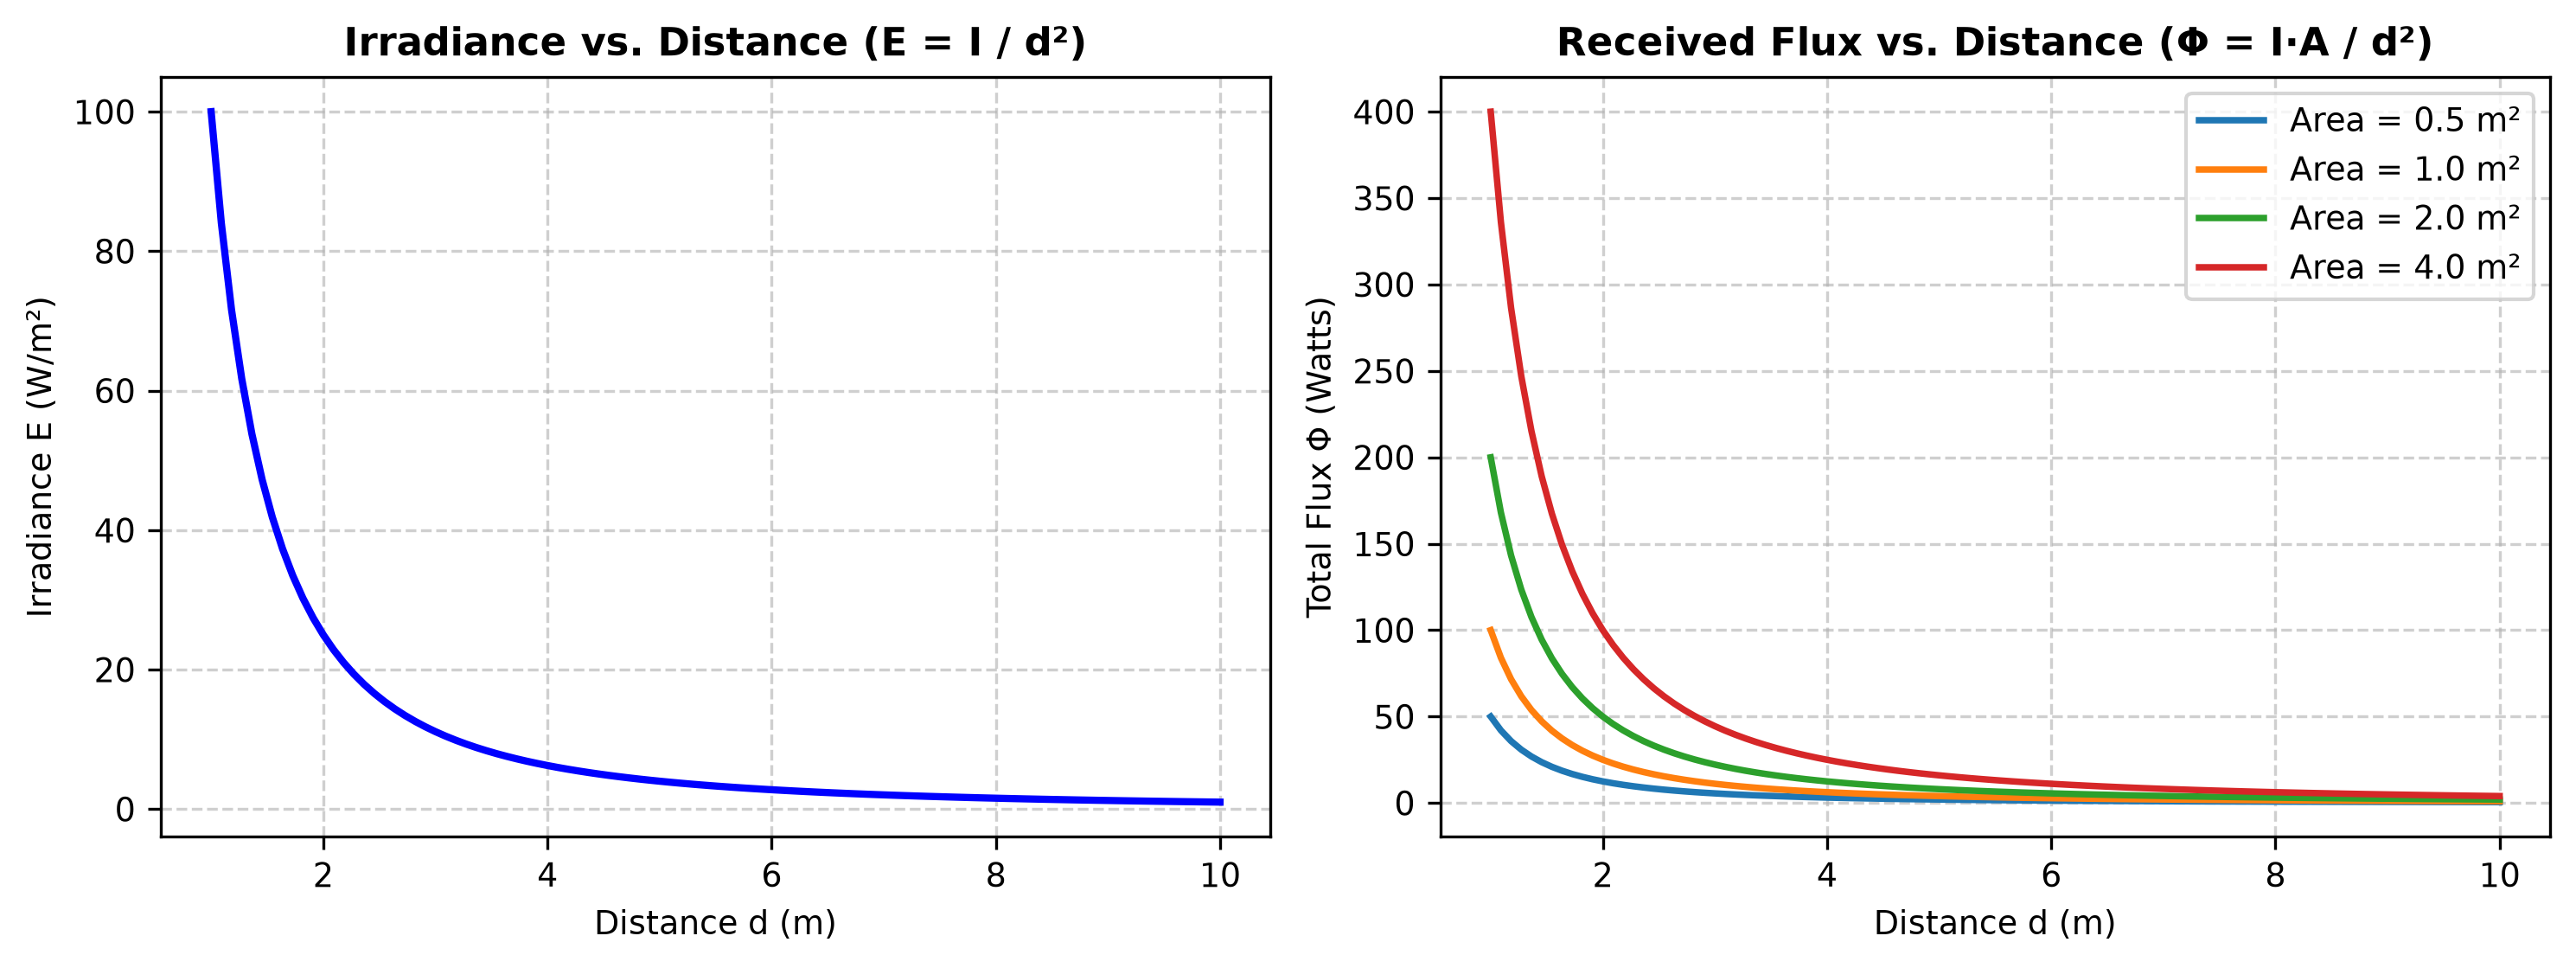
\includegraphics[width=0.82\textwidth]{figures/q1_illumination.png}
    \caption{Received irradiance and total flux vs. distance for various surface areas.}
\end{figure}

\textbf{Observations:}
\begin{itemize}
    \item Irradiance $E$ is completely independent of the receiver area and decreases quadratically ($1/d^2$) with distance.
    \item Total received power $\Phi$ scales linearly with receiver surface area $A$ while preserving the inverse-square distance falloff.
\end{itemize}

% --------------------------------------------------------------
\subsection*{2. Sensitivity Analysis of Received Intensity}
\textbf{Principle:} The intensity received by an arbitrary planar patch depends on source power $P$, distance $d$, surface orientation angle $\theta$ relative to surface normal $\mathbf{N}$, and surface reflectance $\rho$:
\begin{equation}
E = \frac{P \cdot \rho}{4\pi d^2} \cos\theta \quad (\text{for } 0 \le \theta \le \pi/2)
\end{equation}
We evaluate the isolated sensitivity of each factor by sweeping one parameter while holding the others at baseline ($P=100\,\text{W}, d=2\,\text{m}, \theta=0^\circ, \rho=0.8$).

\begin{lstlisting}[style=code]
def calc_intensity(P, d, theta, rho):
    return (P * rho * np.maximum(0.0, np.cos(theta))) / (4.0 * np.pi * (d**2))

P_vals = np.linspace(10, 200, 50)
d_vals = np.linspace(1, 10, 50)
theta_vals = np.linspace(0, np.pi/2, 50)
rho_vals = np.linspace(0.1, 1.0, 50)
\end{lstlisting}

\begin{figure}[H]
    \centering
    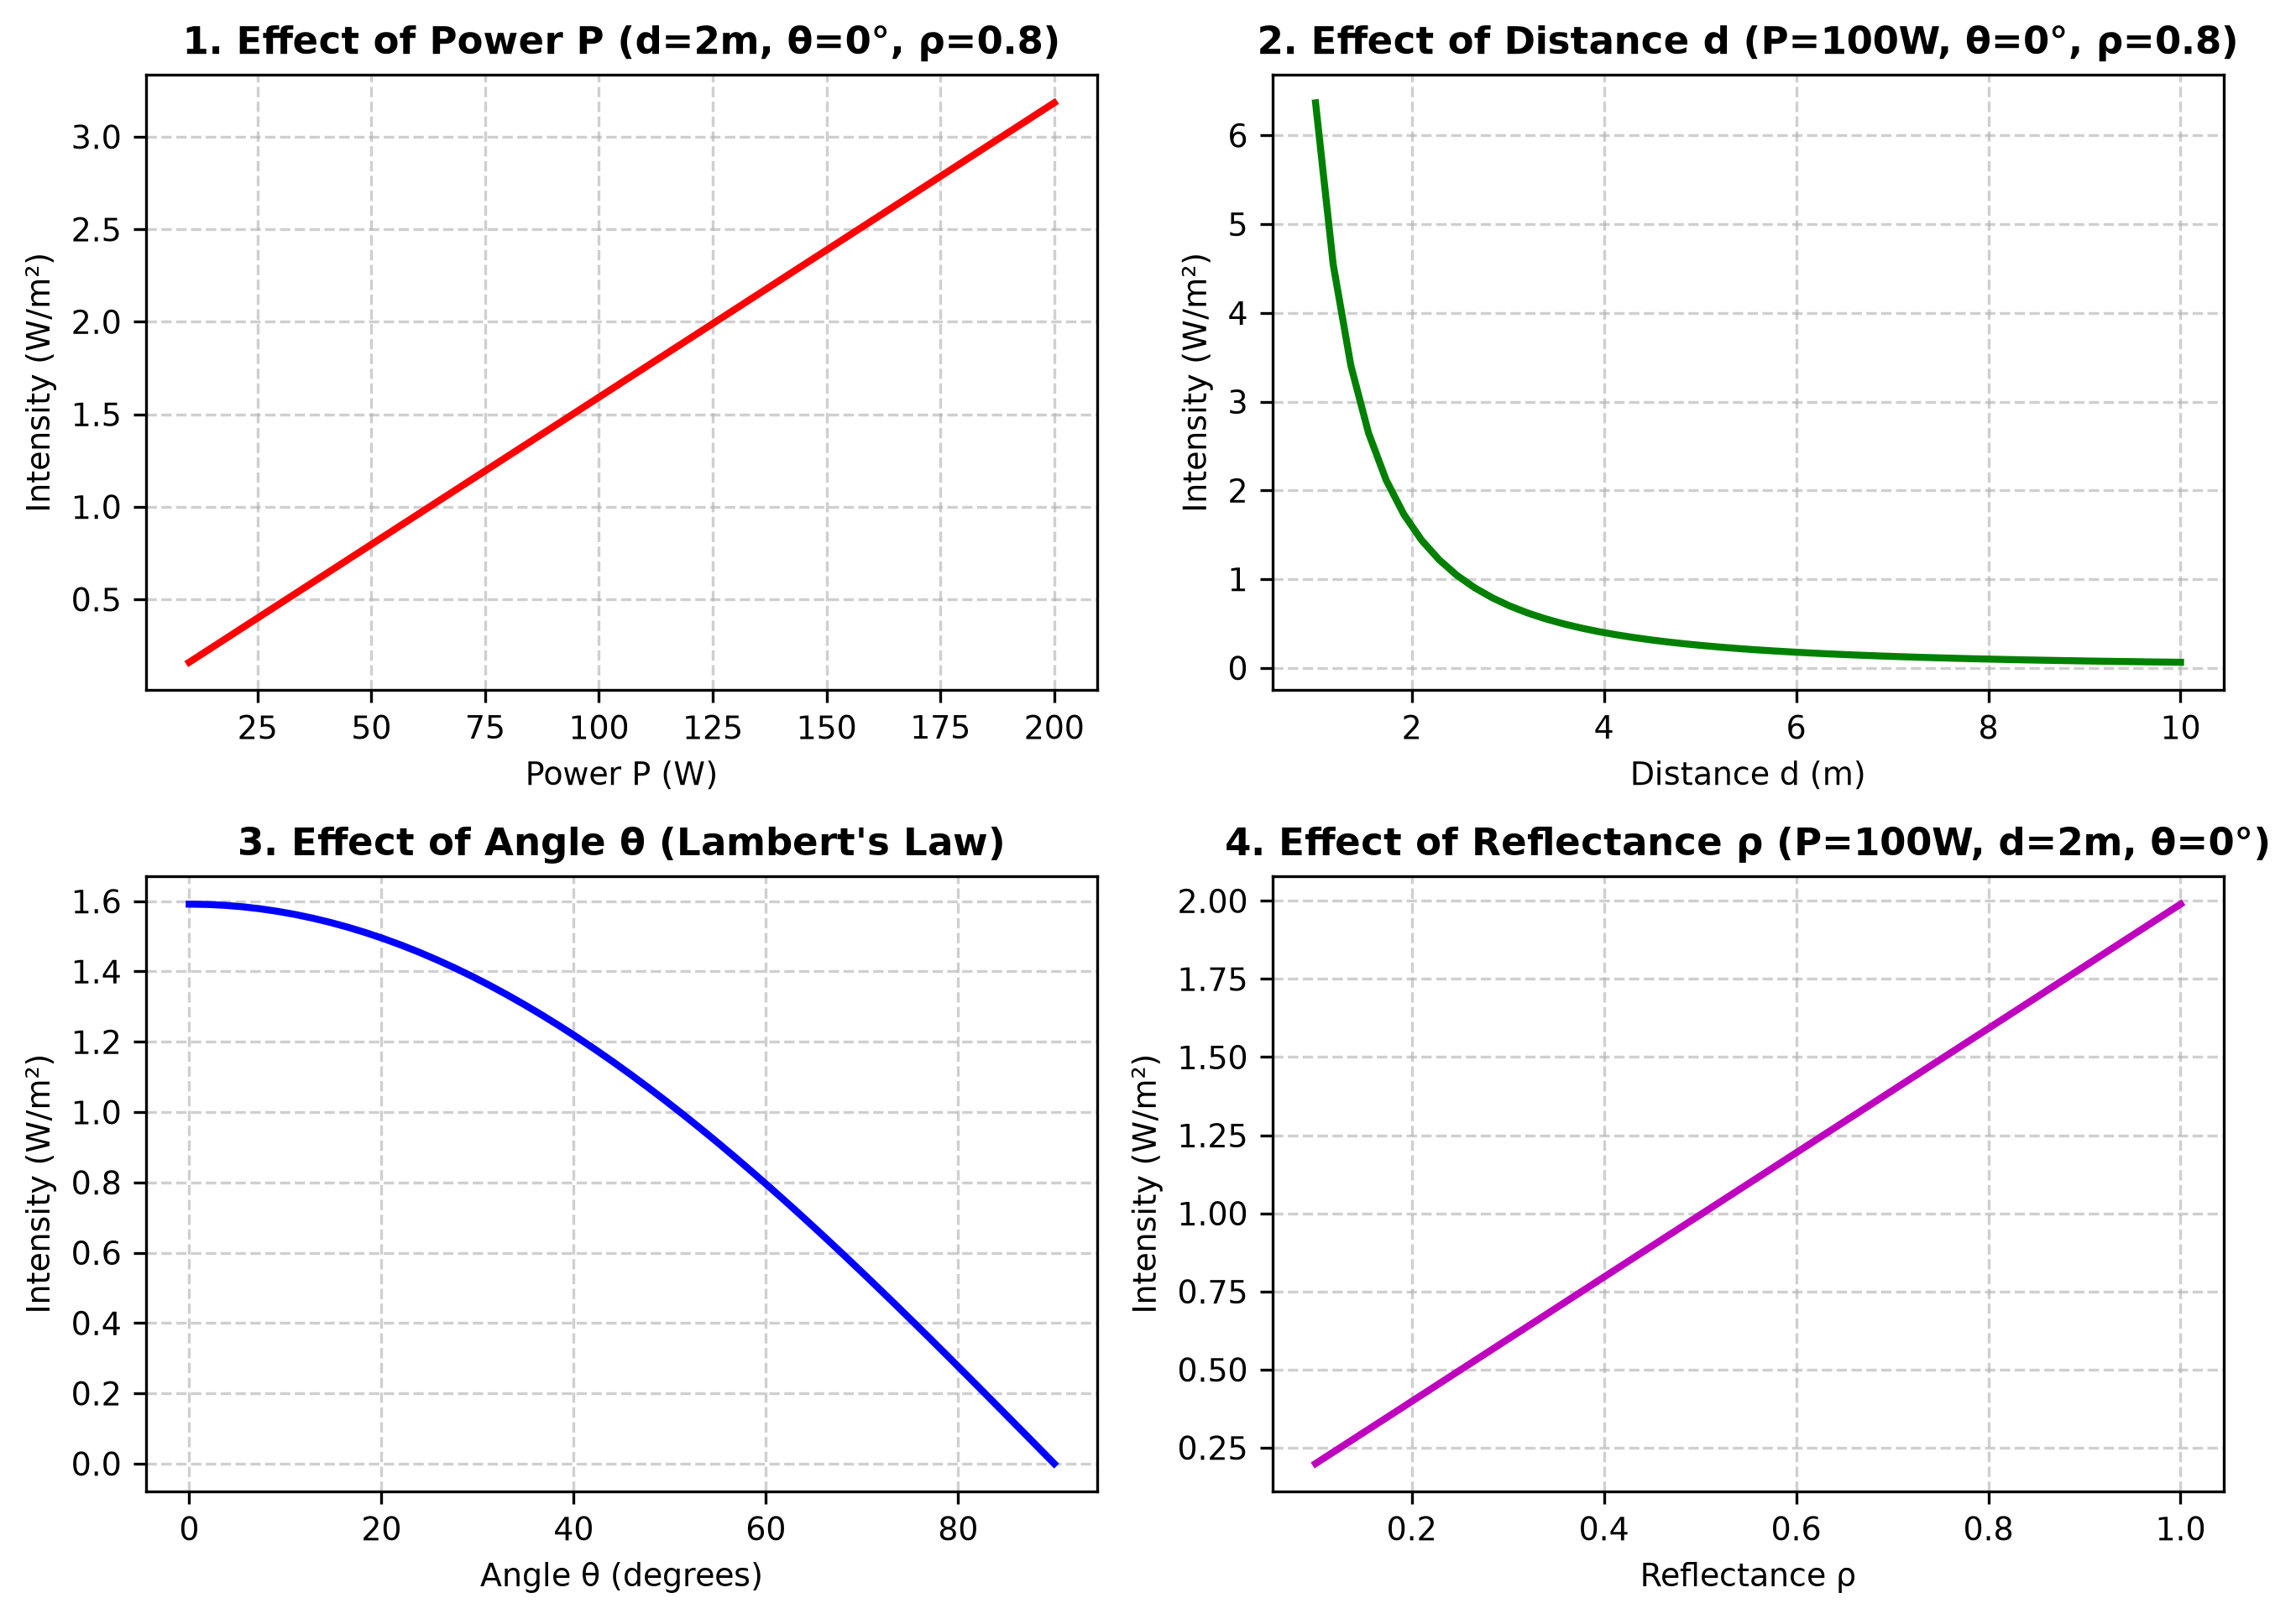
\includegraphics[width=0.75\textwidth]{figures/q2_sensitivity.png}
    \caption{Single-parameter sensitivity analysis of received intensity.}
\end{figure}

\textbf{Observations:}
\begin{itemize}
    \item \textbf{Power ($P$) and Reflectance ($\rho$):} Exhibit direct linear relationships with received intensity.
    \item \textbf{Distance ($d$):} Follows a steep non-linear $1/d^2$ decay.
    \item \textbf{Orientation ($\theta$):} Validates Lambert's Cosine Law; received energy peaks at perpendicular incidence ($\theta=0^\circ$) and drops smoothly to zero at grazing incidence ($\theta=90^\circ$).
\end{itemize}

% --------------------------------------------------------------
\subsection*{3. Diffuse vs. Specular Surface Reflection}
\textbf{Principle:} 
\begin{itemize}
    \item \textbf{Lambertian Diffuse Surface:} Outgoing radiance is isotropic and view-independent: $I_{\text{diff}} = k_d (\mathbf{N} \cdot \mathbf{L}) = k_d \cos\theta_L$.
    \item \textbf{Specular (Phong) Surface:} Produces directional highlight concentrated around the perfect reflection vector $\mathbf{R}$: $I_{\text{spec}} = k_a + k_s (\mathbf{R} \cdot \mathbf{V})^\alpha$, where $\alpha$ is surface shininess.
\end{itemize}

\begin{lstlisting}[style=code]
view_angles = np.linspace(-np.pi/2, np.pi/2, 200)
theta_L = np.radians(35)  # Light incident at 35 degrees
kd, ks, alpha = 0.8, 0.85, 20

I_diffuse = np.full_like(view_angles, kd * max(0.0, np.cos(theta_L)))
cos_RV = np.maximum(0.0, np.cos(view_angles - theta_L))
I_specular = (0.15 * max(0.0, np.cos(theta_L))) + ks * (cos_RV ** alpha)
\end{lstlisting}

\begin{figure}[H]
    \centering
    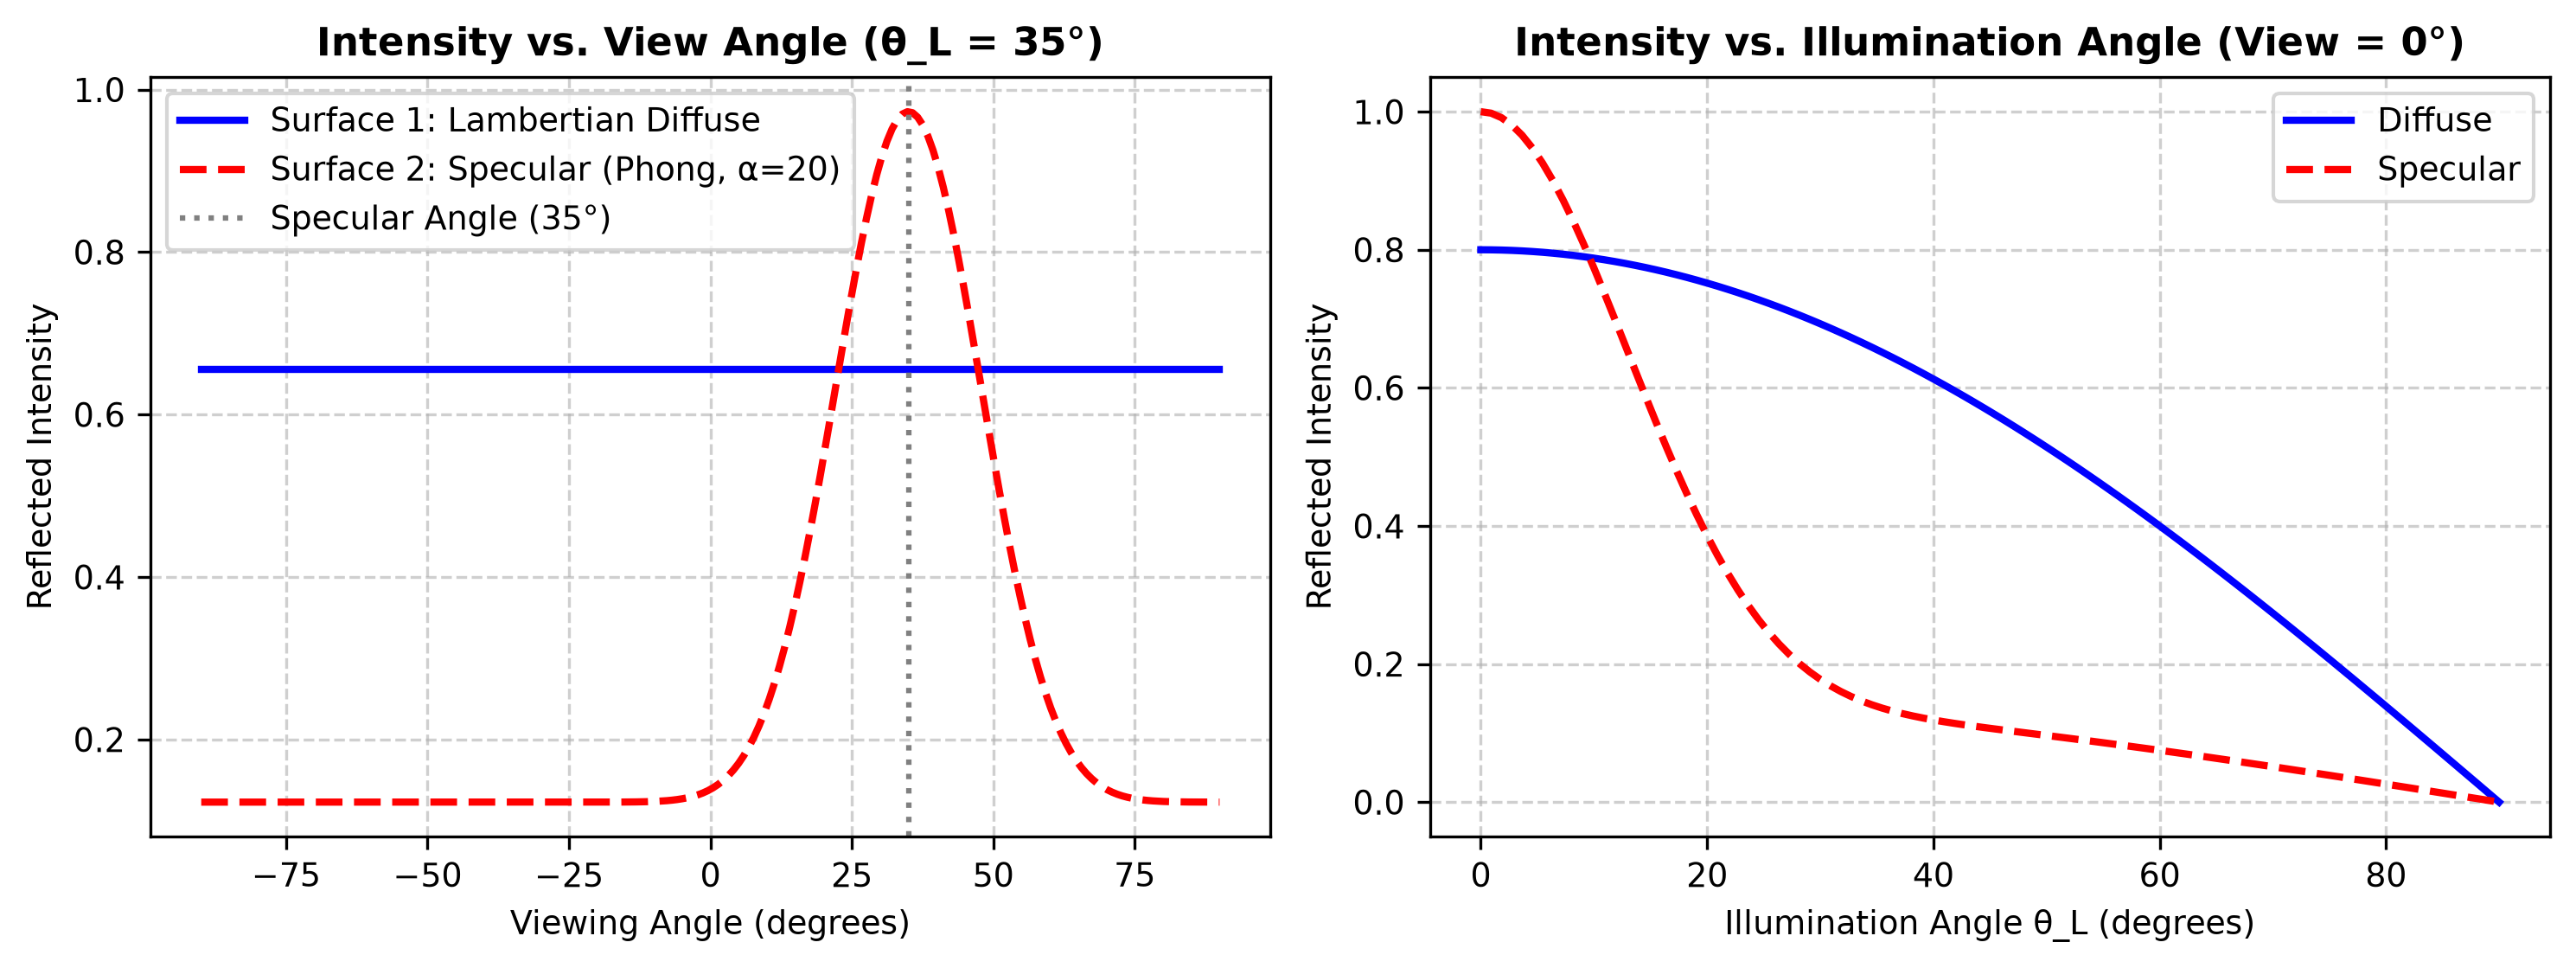
\includegraphics[width=0.82\textwidth]{figures/q3_reflection.png}
    \caption{Reflected intensity comparison across viewing and illumination angles.}
\end{figure}

\textbf{Observations:}
\begin{itemize}
    \item The diffuse surface maintains constant brightness regardless of viewing angle $\theta_V$.
    \item The specular surface produces an intense highlight lobe centered precisely at the reflection angle $\theta_V = 35^\circ$.
\end{itemize}

\textit{Note: Questions 4 and 5 from Part A were omitted as per lab instructions.}

% --------------------------------------------------------------
\subsection*{6. Complete Image-Formation Process Simulation}
\textbf{Principle:} The physical formation of an image converts incident scene light into quantized sensor values:
\begin{equation}
E_0 \xrightarrow{\text{Surface Reflection}} L_o = \frac{\rho}{\pi} E_0 \xrightarrow{\text{Optics}} E_i = L_o \frac{\pi}{4 N^2} \xrightarrow{\text{Sensor ADC}} P = \text{clip}\left(\lfloor g \cdot E_i \cdot \Delta t \rfloor, 0, 255\right)
\end{equation}
where $N=f/D$ is lens f-number, $\Delta t$ is exposure time, and $g$ is sensor gain.

\begin{lstlisting}[style=code]
def simulate_image_formation(E0, rho, is_glossy=False, f_num=2.8, t_exp=0.012, sensor_gain=4500):
    Lo = (rho / np.pi) * E0 * (1.4 if is_glossy else 1.0)
    Ei = Lo * (np.pi / 4.0) * (1.0 / (f_num ** 2))
    raw_val = sensor_gain * Ei * t_exp
    return np.clip(np.round(raw_val), 0, 255).astype(int)
\end{lstlisting}

\begin{figure}[H]
    \centering
    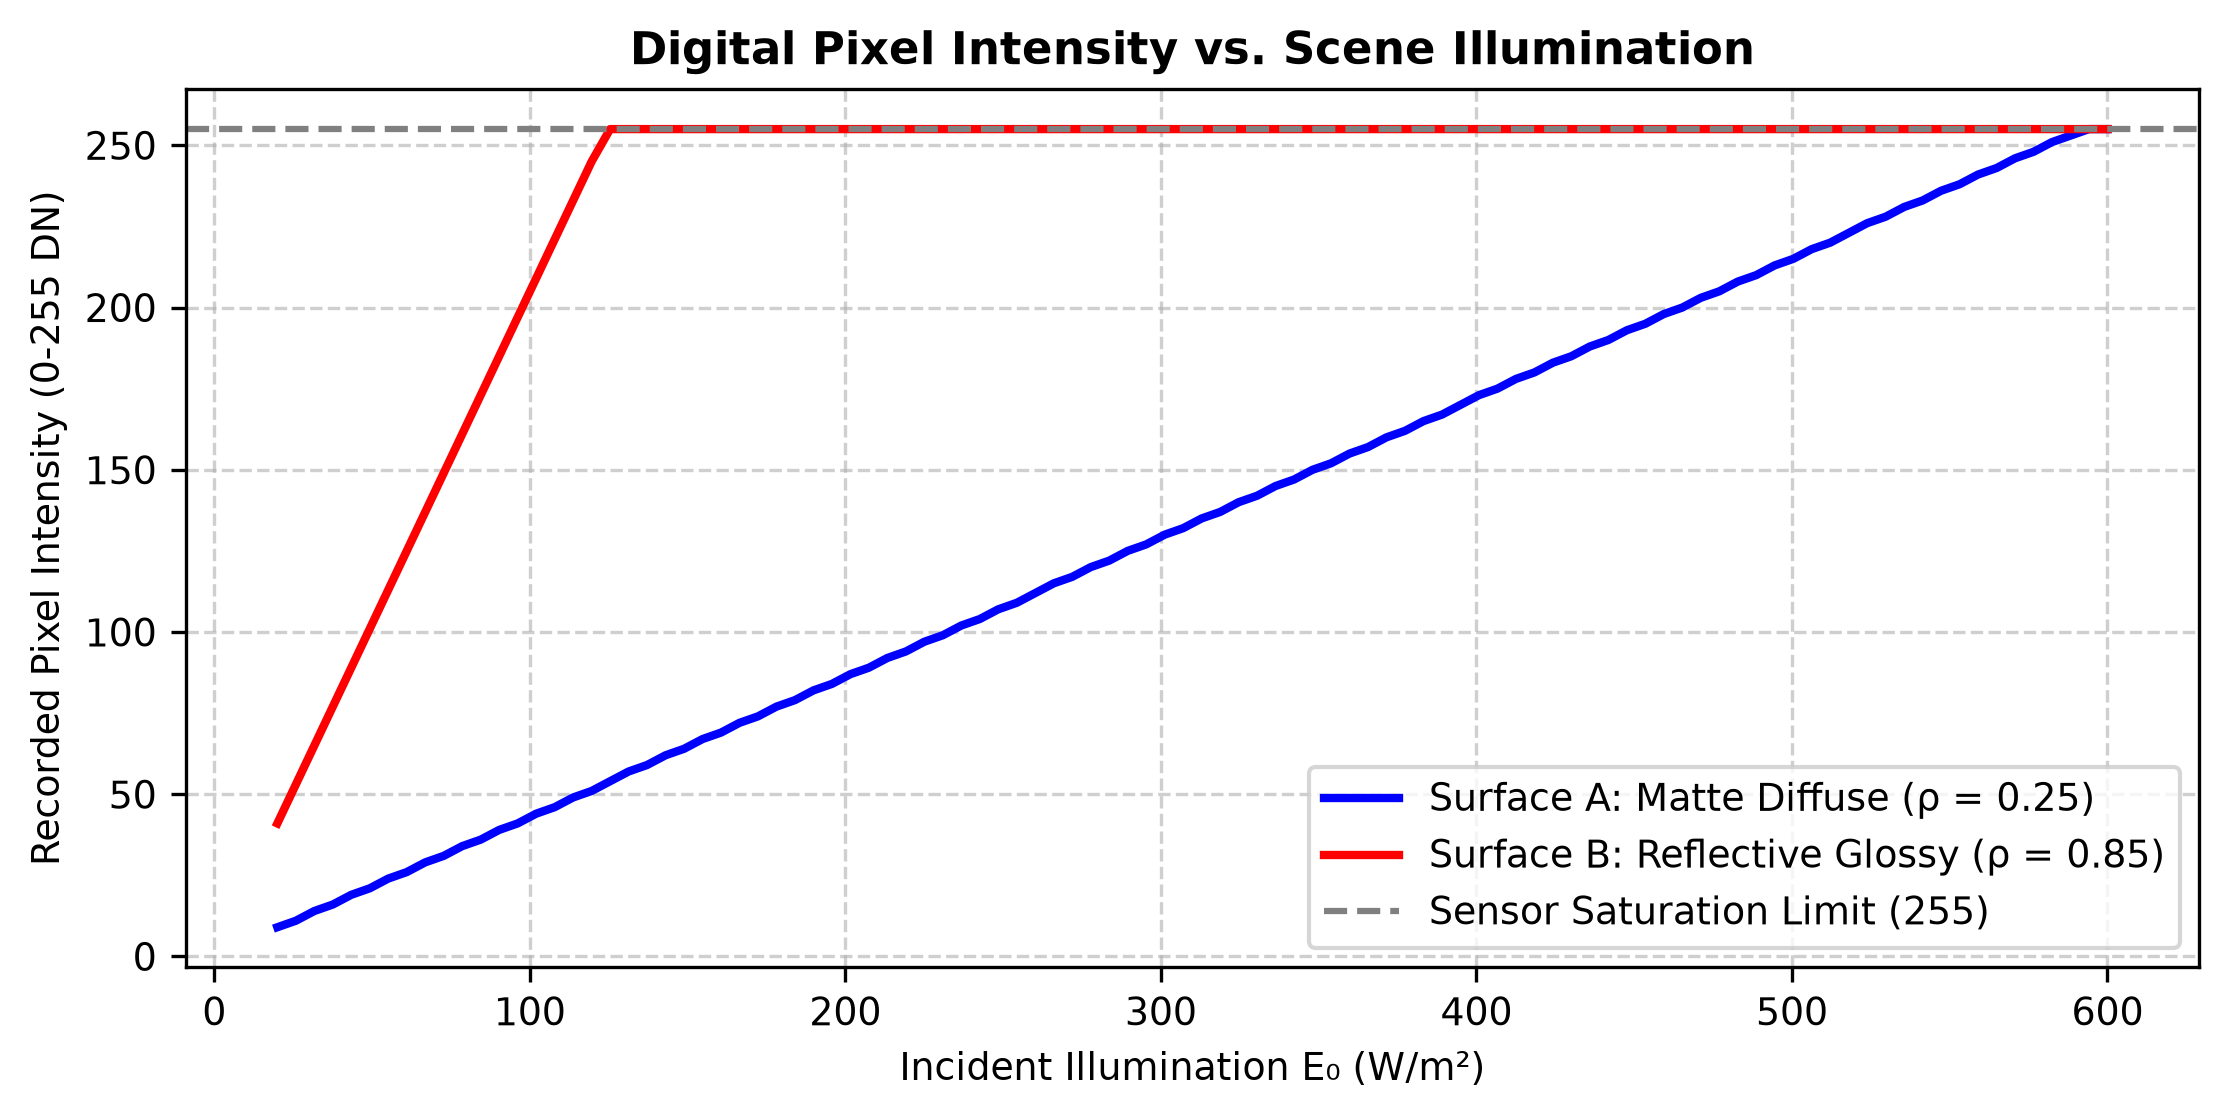
\includegraphics[width=0.68\textwidth]{figures/q6_pipeline.png}
    \caption{Digitized pixel intensity vs. scene illumination for matte and glossy surfaces.}
\end{figure}

\textbf{Observations:}
\begin{itemize}
    \item The sensor exhibits a linear response region until reaching the 8-bit saturation cap of 255.
    \item The highly reflective glossy surface reaches full saturation at a significantly lower illumination threshold ($\sim 250\,\text{W/m}^2$) than the matte surface ($\sim 580\,\text{W/m}^2$).
\end{itemize}

% --------------------------------------------------------------
\subsection*{7. Synthetic Scene Under Different Illumination Conditions}
\textbf{Setup:} A synthetic 3D hemispherical object resting on a planar floor is rendered under two illumination configurations:
\begin{enumerate}
    \item \textbf{Direct Overhead Light:} Light vector $\mathbf{L}_1 = [0, 0, 1]^T$ produces symmetric shading.
    \item \textbf{Oblique Side Light:} Light vector $\mathbf{L}_2 = [-0.75, -0.2, 0.63]^T$ produces strong directional highlights and long cast shadows.
\end{enumerate}

\begin{figure}[H]
    \centering
    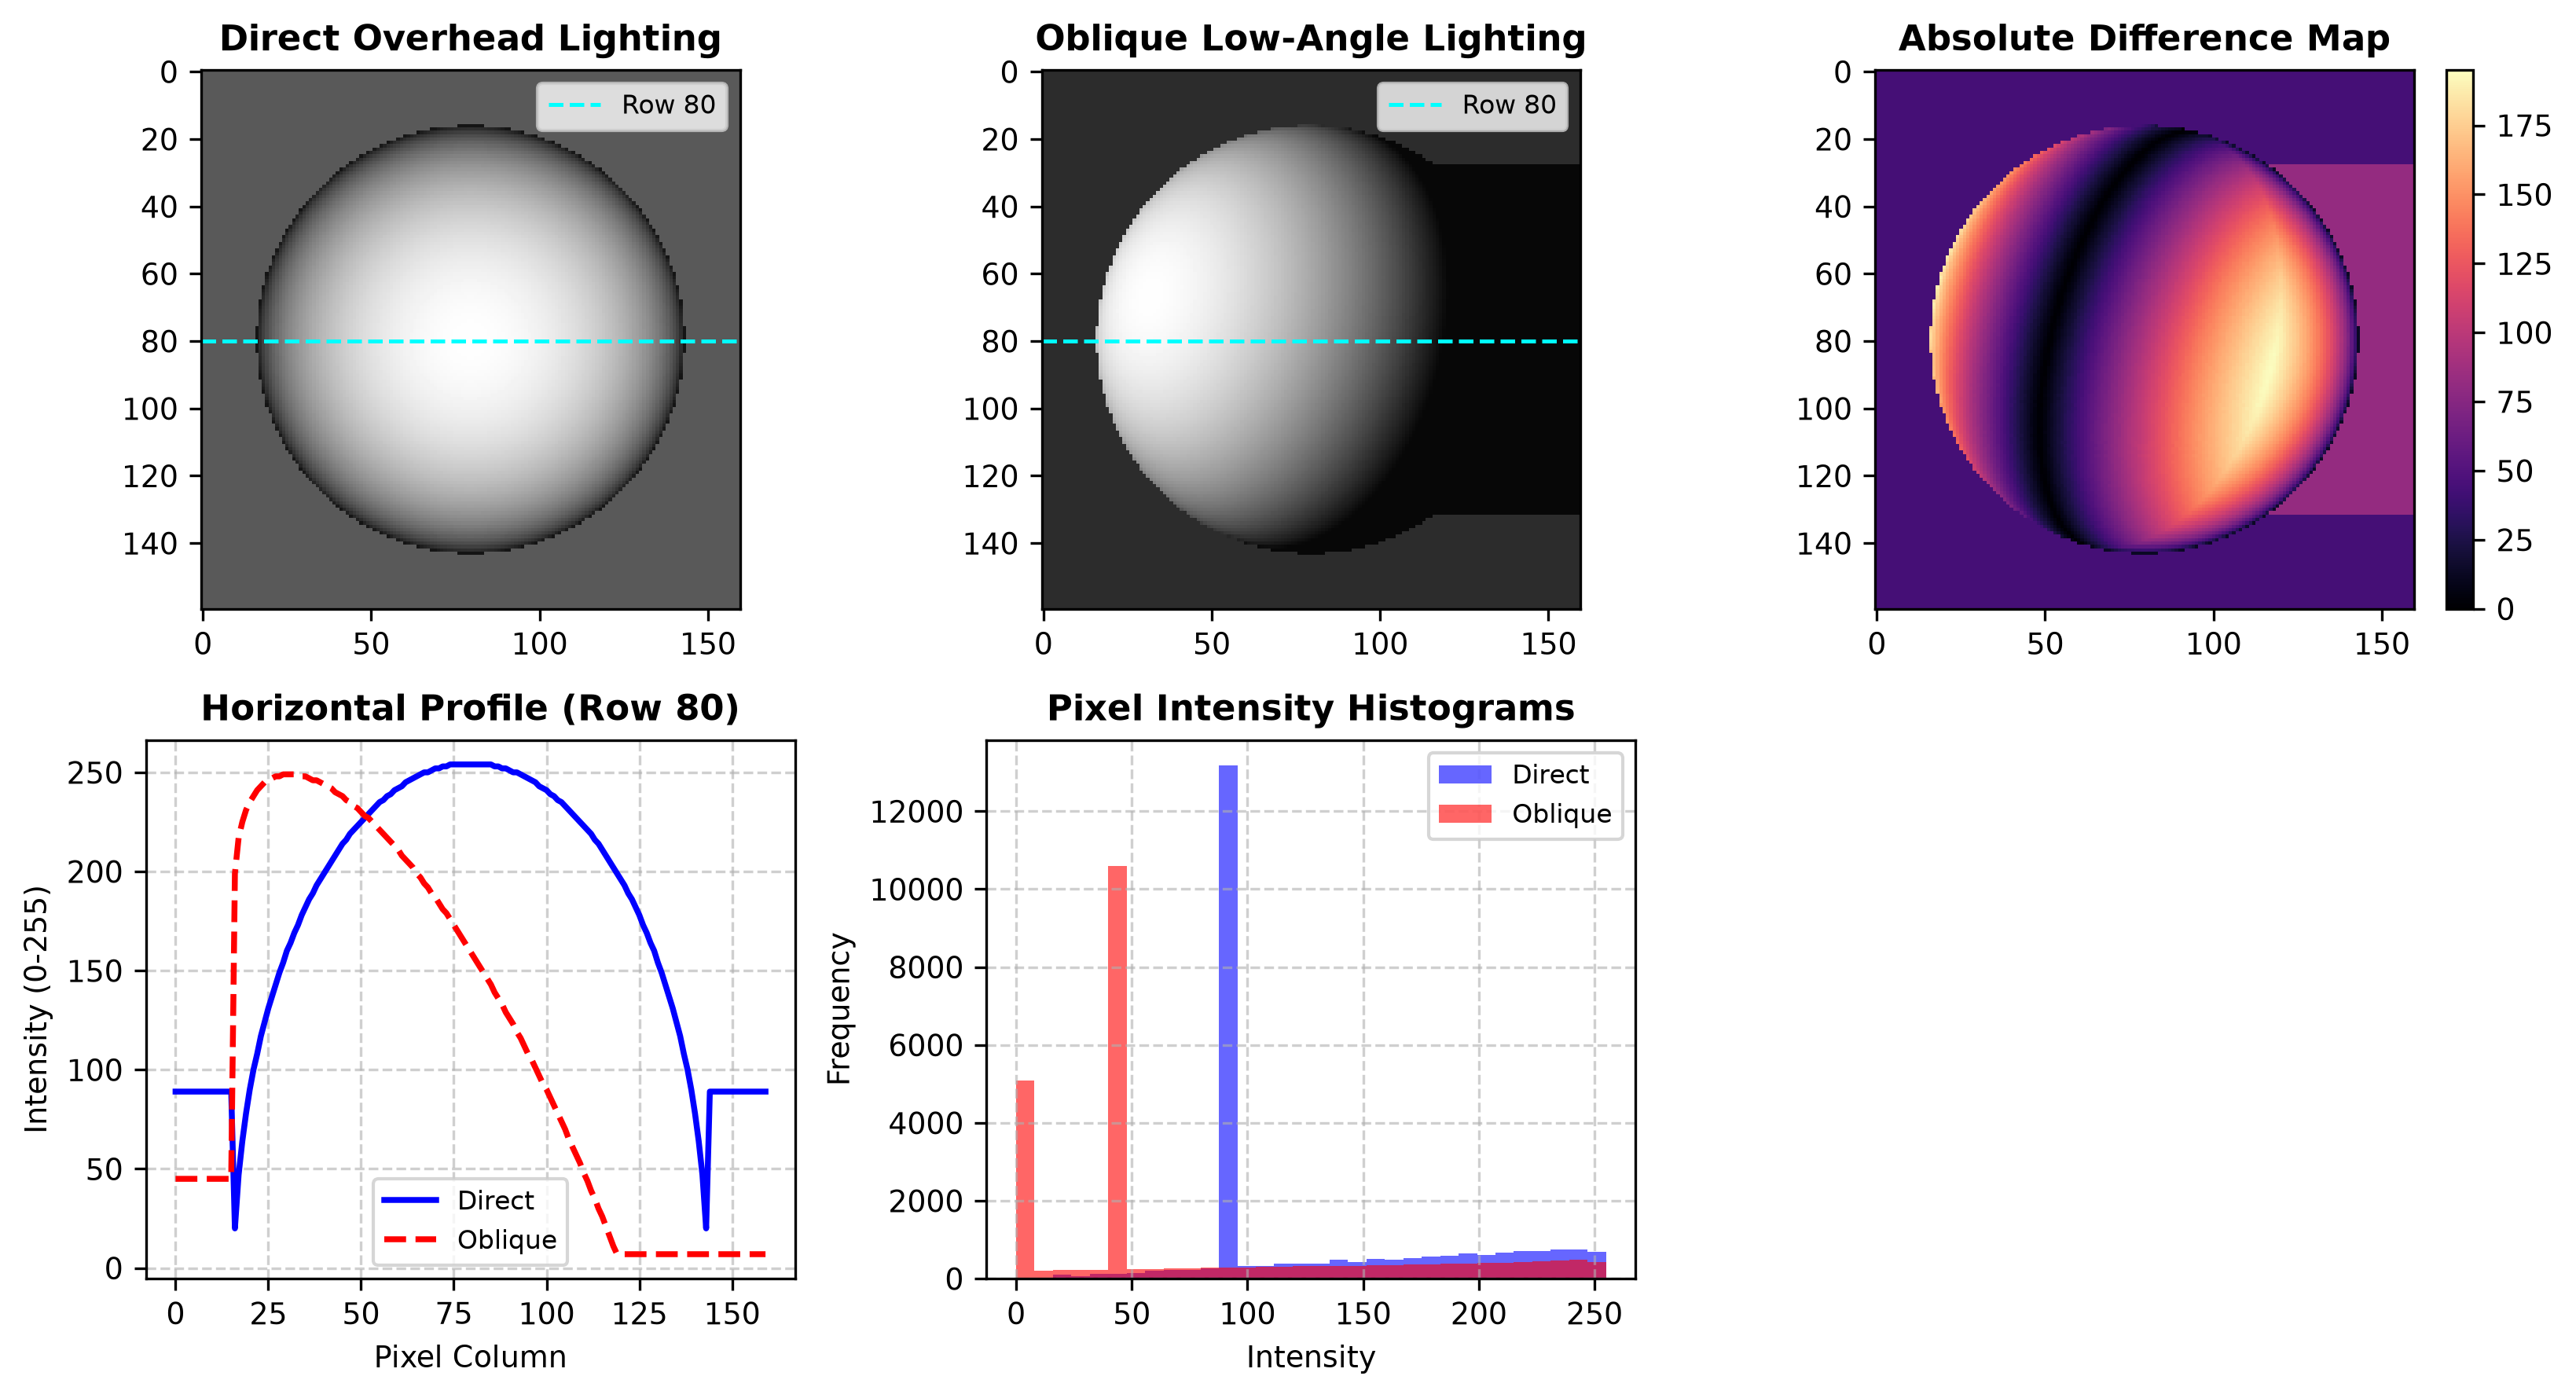
\includegraphics[width=0.88\textwidth]{figures/q7_synthetic_scene.png}
    \caption{Synthetic scene comparison: images, difference map, profile slice, and histograms.}
\end{figure}

\textbf{Observations:}
\begin{itemize}
    \item \textbf{Intensity Profile (Row 80):} The direct overhead case is symmetric and smooth, whereas the oblique lighting profile shows a steep gradient on the illuminated side and drops to shadow levels on the opposite side.
    \item \textbf{Histograms:} Direct lighting creates a unimodal distribution centered at mid-to-high values; oblique lighting produces a heavily bimodal/skewed distribution due to background shadows and localized highlights.
\end{itemize}

% ==============================================================
\section*{Part B: Experimental Investigation}
% ==============================================================

\subsection*{Direct Illumination vs. Shadow Comparison}
An object was captured under two contrasting lighting regimes:
\begin{itemize}
    \item \textbf{Direct Illumination:} Direct line-of-sight irradiance from the primary emitter.
    \item \textbf{Shadowed Condition:} Direct light occluded; illumination provided solely by indirect ambient scatter.
\end{itemize}

\subsubsection*{Statistical Metrics Comparison}
\begin{lstlisting}[style=output]
==============================================================
PART B: STATISTICAL METRICS COMPARISON
==============================================================
Condition            | Mean Intensity | Std Deviation
--------------------------------------------------------------
Direct Illumination  |         129.00 |         58.37
Shadowed Condition   |          27.42 |         25.64
==============================================================
\end{lstlisting}

\begin{figure}[H]
    \centering
    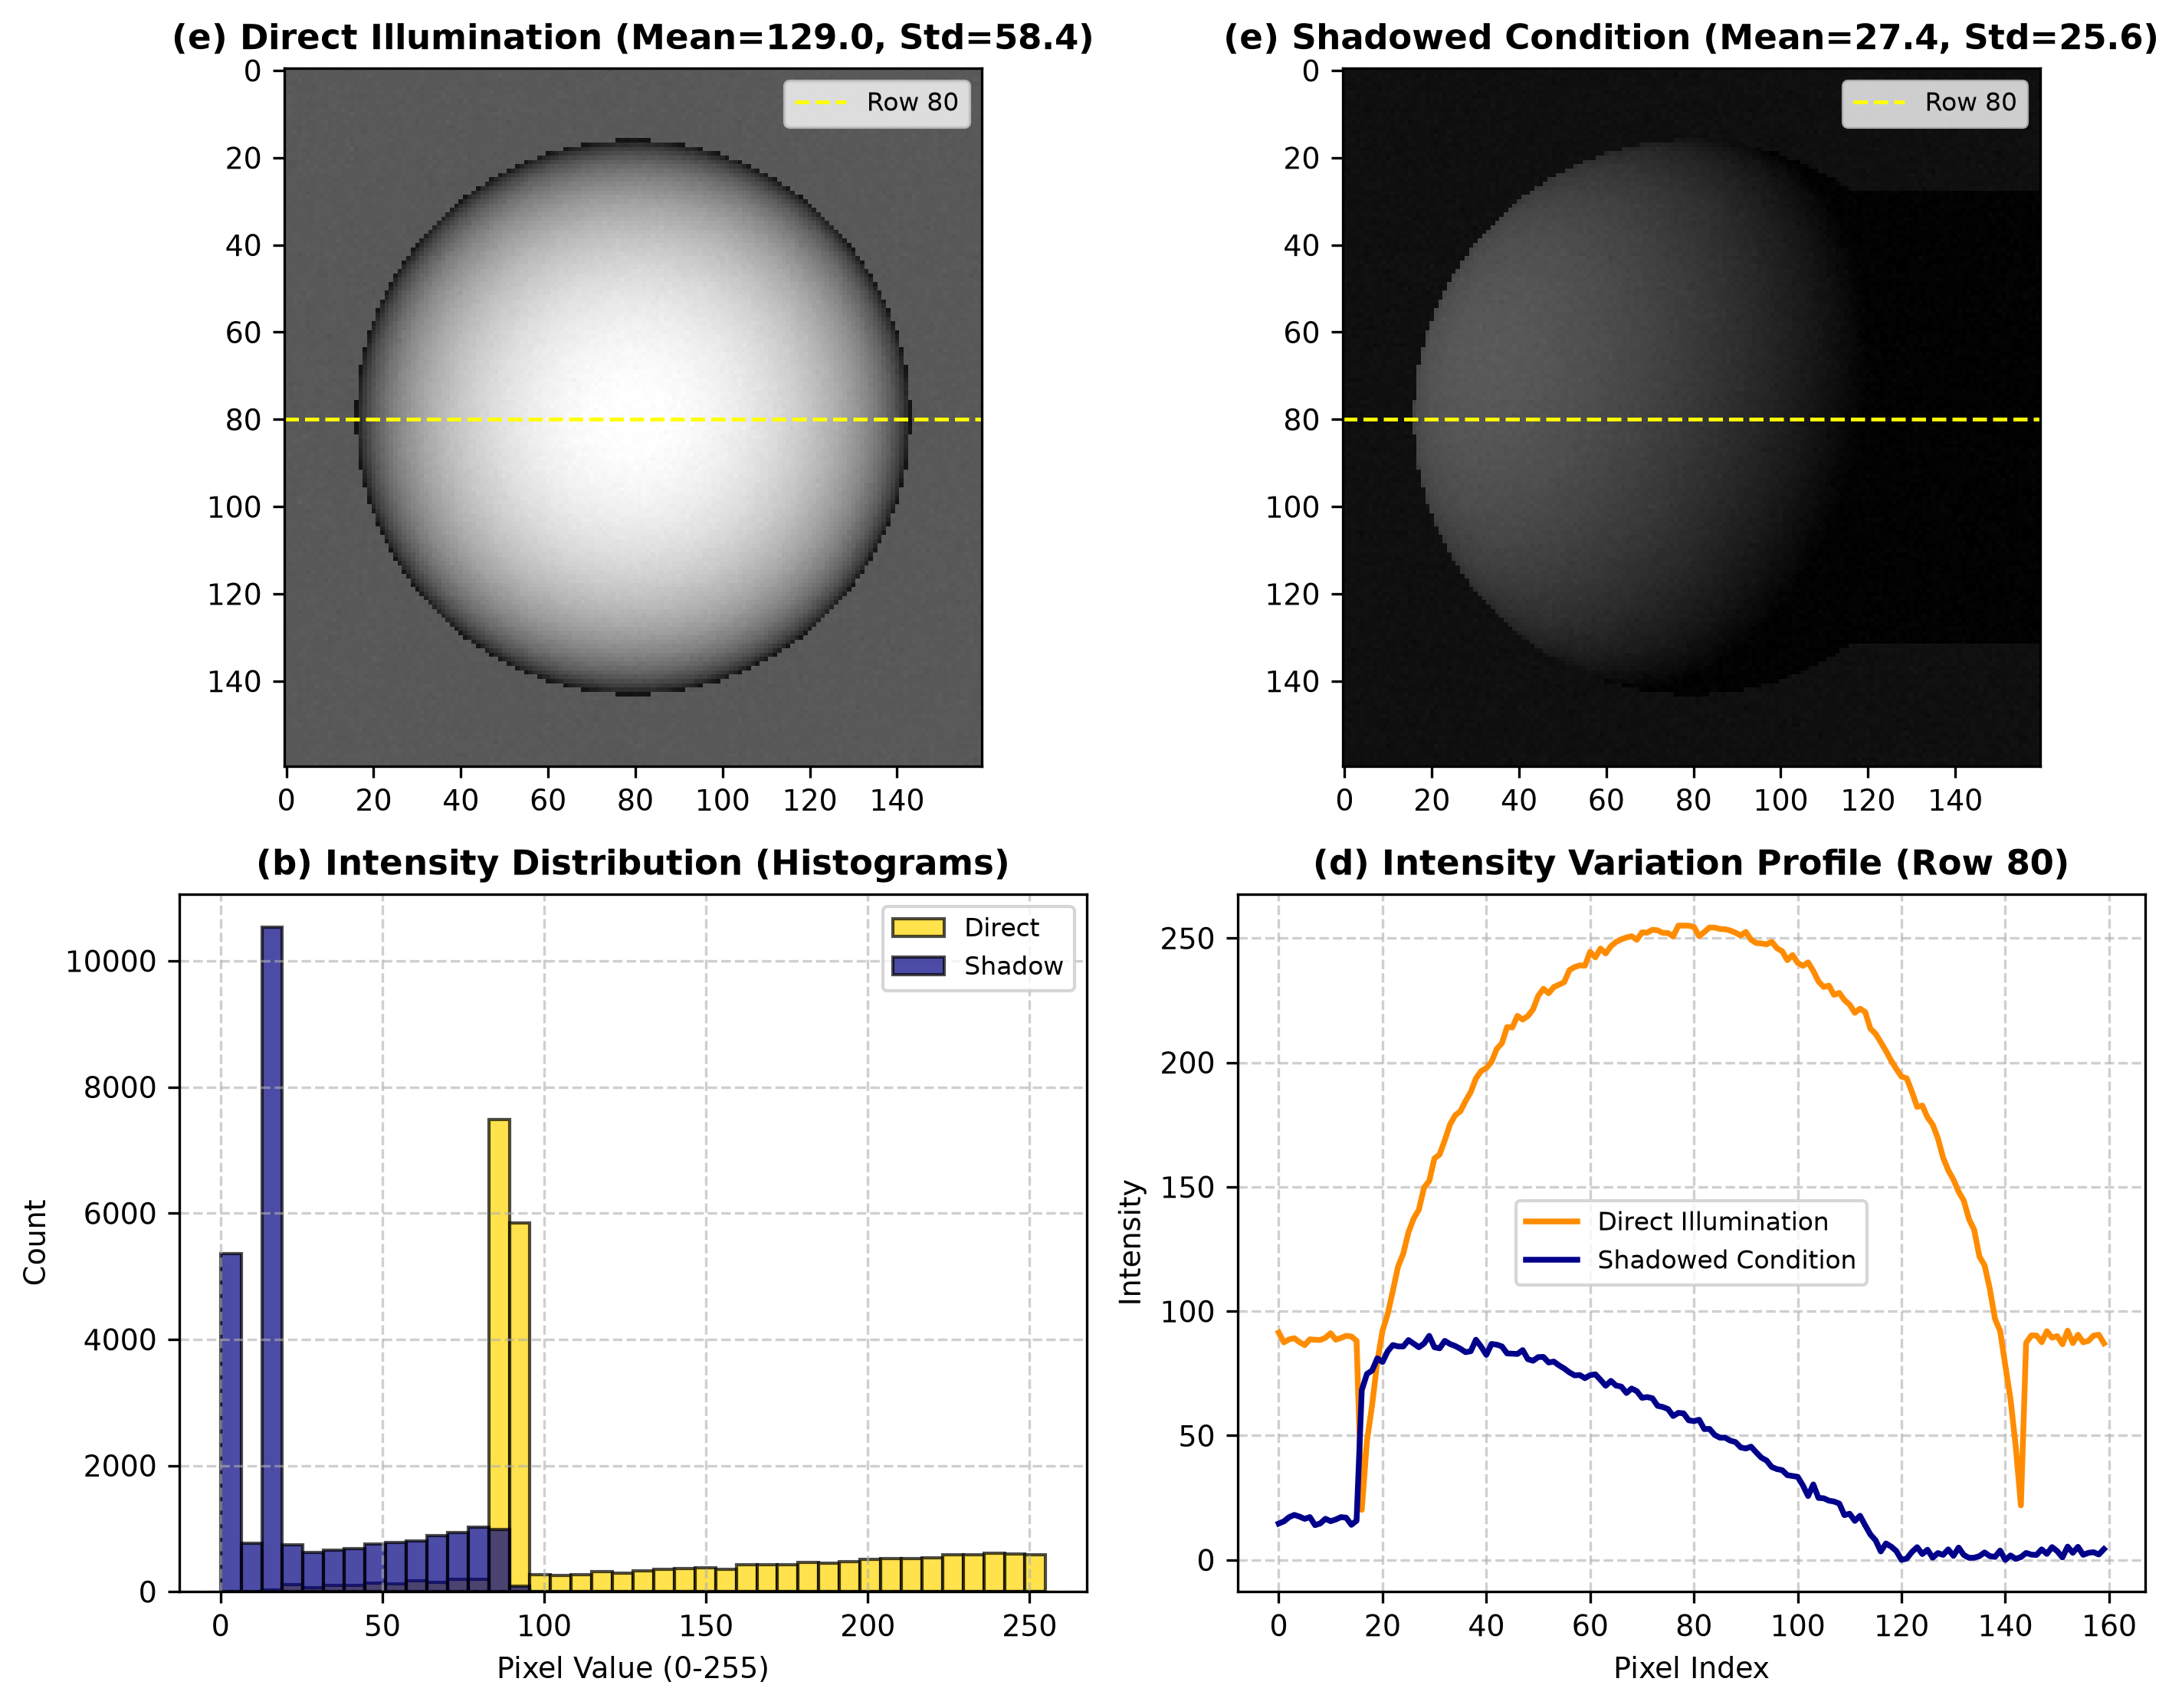
\includegraphics[width=0.82\textwidth]{figures/part_b_investigation.png}
    \caption{Experimental comparison of direct illumination vs. shadow.}
\end{figure}

\subsubsection*{Detailed Evaluation and Physical Image-Formation Insights}
\begin{enumerate}
    \item[(a)] \textbf{Overall Brightness:} Direct illumination yields an average brightness of $129.00\,\text{DN}$, whereas the shadowed scene averages only $27.42\,\text{DN}$ (an $\sim 80\%$ brightness drop).
    \item[(b)] \textbf{Pixel-Intensity Distribution:} The direct histogram is broad and spans the dynamic range up to $255\,\text{DN}$. The shadow histogram is tightly clustered between $0$ and $50\,\text{DN}$.
    \item[(c)] \textbf{Mean and Standard Deviation:} The standard deviation under direct light is $58.37\,\text{DN}$ (rich visual contrast) versus $25.64\,\text{DN}$ in shadow (low contrast, flattened detail).
    \item[(d)] \textbf{Intensity Variation Across Selected Regions:} Across Row 80, the direct profile demonstrates strong geometric modulation driven by $\mathbf{N} \cdot \mathbf{L}$, whereas the shadow profile is compressed and flat.
    \item[(e)] \textbf{Visible Changes \& Underlying Image Formation Factors:}
    \begin{itemize}
        \item \textbf{Incident Irradiance ($E$):} Shadows receive only secondary ambient diffuse scatter, drastically cutting the available photons at the lens aperture.
        \item \textbf{Orientation Shading ($\cos\theta$):} Under direct collimated light, 3D shape cues emerge strongly via Lambertian shading. Under shadow, diffuse ambient illumination illuminates all directions uniformly, suppressing geometric gradients.
        \item \textbf{Sensor Dynamic Range \& SNR:} Shadowed areas occupy the lower quantization bins where sensor read noise represents a larger fraction of the signal, reducing the effective Signal-to-Noise Ratio (SNR).
    \end{itemize}
\end{enumerate}

\end{document}
